\documentclass[12pt]{article}
\usepackage{bm}
\usepackage{subfigure}
\usepackage{fullpage}
\usepackage{enumerate}
\usepackage{graphicx}
\usepackage{graphics}
\usepackage{comment}
\usepackage{amsmath,amssymb,amsfonts,amsthm}
\usepackage{bbm}
\usepackage{setspace}
\usepackage{verbatim}
\usepackage[authoryear]{natbib}
%\usepackage{mathabx}
%\usepackage{filecontents}
%\usepackage{bibentry}
%\usepackage{hanging}
%\usepackage{apacite}

\doublespacing
\newcommand{\xch}{\check{X}}
\newcommand{\g}{g}
\newcommand{\st}{\mathcal{R}}
%\newcommand{\ych}{$\check{Y}$}
%\newcommand{\ych}{\check{Y}}
\newcommand{\ych}{E}
\newcommand{\yci}{$Y_{Ci}$}
\newcommand{\yti}{$Y_{Ti}$}
\newcommand{\ycim}{Y_{Ci}}
\newcommand{\ytim}{Y_{Ti}}
%\newcommand{\Xi}{$X_{i}$}
\newcommand{\xperp}{$X^\bot$}
\newcommand{\xpar}{$X^\parallel$}
%\newcommand{\E}{\mathop{\bf E\/}}
\newcommand{\E}{\mathbb{E}}
\newcommand{\indicator}[1]{\mathbbm{1}_{\left[ {#1} \right] }}
\newcommand{\yhati}{\hat{Y}_i}
\newcommand\independent{\protect\mathpalette{\protect\independenT}{\perp}}
\newcommand\hsg{$hsgrade\_pct$}
\newcommand\hsgm{hsgrade\_pct}
\newcommand{\tpb}{\hat{\tau}_{PBP}}
%\newcommand\verb|xBalance()|{\verb| xBalance() |}
\newcommand{\hyp}{H_{\bm{\phi_0}}}
\newcommand{\ychphib}{\bm{\check{Y}_{\phi_0}}}
\newcommand{\ychphi}{\check{Y}_{\bm{\phi_0}i}}

\def\independenT#1#2{\mathrel{\rlap{$#1#2$}\mkern2mu{#1#2}}}
\newtheorem{conjecture}{Conjecture}
\newtheorem{ce}{Counter-Example}
%\newtheorem{ass}{Assumption}
\newtheorem{alg}{Algorithm}
%\newtheorem*{ass*}{Assumption}
\newtheorem{prop}{Proposition}
\newtheorem{lemma}{Lemma}

\newenvironment{ass}[2][Assumption]{\begin{trivlist}
\item[\hskip \labelsep {\bfseries #1}\hskip \labelsep ({\bfseries #2}).]}{\end{trivlist}}



\title{Limitless Regression Discontinuity}

\usepackage{Sweave}
\begin{document}
\maketitle

\section{Introduction}

Randomization of treatment assignment is the gold-standard of causal
inference in statistics: it is the only sure way to control all confounding.
Of the options available when experiments are impossible, the
``regression discontinuity design" (RDD)
\citep{thistlethwaite1960regression,cook2008waiting,imbens2008regression,lee2010regression}
is among the most credible.
In an RDD, the treatment assignment mechanism is known: each subject
$i$ has a ``running variable'' $R_i$, and those subjects whose $R_i$
is greater (or less) than a pre-determined constant $c$ are assigned
to treatment.
\citet{lee2008randomized} argued
that the RDD features ``local randomization" of treatment assignment,
and is therefore ``a highly credible and transparent way of estimating
program effects" \citep[][p. 282] {lee2010regression}.

Lee's notion of local randomization is that, in a well-behaved RDD,
one can recover the important advantages of randomized
experiments---specifically, no confounding, unbiased estimation of
average treatment effects (ATE) and covariate balance---by replacing
statements about samples or populations with statements about limits.
In one telling \citep{imbens2008regression}, the target estimand is the average effect of the treatment in the region around the cutoff that is the limit of concentric ever-shrinking regions---esentially an infinitesimal interval. 
%For instance, in a randomized experiment a covariate $X$ has the same
%distribution regardless of treatment assignment.
%In an RDD, the distribution of $X$, as a function of $R$, is
%continuous at the cutoff $c$.
%That is, the limits of $X$'s distribution, as $R$ approaches $c$ from
%both sides, are identical.
The conventional approach to RDDs
\citep[eg.][]{berk1983capitalizing,angrist1999using,oreopoulos2006estimating}, consistent with this ``limit'' understanding,
uses regression to estimate the average functional
relationship between the outcomes $Y$, the running variable $R$ and
treatment assignment $Z$.

However, formulating local randomization in terms of limits fails to
realize some other benefits of experiments.
In particular, randomized experiments allow researchers to estimate
treatment effects for specific samples or
sub-populations.
In contradistinction, conventional RDD analysis estimates an
ambiguously weighted population ATE \citep[as
in][]{lee2008randomized}, or the limit of
sample ATEs as sub-populations shrink around a cutoff \citep[as
in][]{hahn2001identification}.
Similarly, randomized experiments allow analysts access to
distribution-free inferential methods, equally valid for large or
small samples
\citep{fisher:1935,pitman1937significance,rosenbaum:2002}.
%These assets would
%accompany a more literal interpretation of local randomization: that,
%in a window around $c$, treatment assignment is random or ignorable
%\citep[cf.][]{rubin:1978}.

This paper will suggest a method of modeling RDDs that realizes these
benefits while also retaining some of the flavor of the conventional
approach, using regression techniques to disentangle $Y$ and $R$.
The new approach has several advantages over the conventional approach.
Its assumptions align better with the heuristic motivation that RDDs
leverage natural randomization in the vicinity of a cut point.
Since it relies on exact inference or permutation tests, it is
suitable for small-sample inference.
Similarly, the conceptual approach does not demand continuity in the
running variable $R$, since it does not rely on taking limits of
continuous functions of $R$.
In fact, the data example we discuss below features a discrete $R$,
which poses conceptual difficulties for the conventional approach.

The new approach allows the use of covariate adjustment not only to make
estimates more precise but also to expand the notion of ``local.''
That is, it estimates the treatment effect in a broader sample.
Similarly, it suggests testable consequences of the model that can be
wholly separate from estimation of treatment effects.
In some scenarios, it allows researchers to use those consequences to
make improvements to the model that would be incompatible with the
conventional, limit-focused approach.

Our RDD analysis strategy unites the conventional, regression-based
approach, with a randomization-based approach, as advanced primarily
in \citet{rocio}.
Briefly, the idea is to use regression modeling to disentangle the
outcome from the running variable, producing ``transformed'' outcomes
that are hopefully independent of treatment assignment, as
(un-transformed) outcomes would be in an experiment.
Then, use randomization inference techniques to test for, and
estimate, an effect.

Like the conventional approach, it models outcomes and treatment
effects as functions of the running variable, and typically fits these
models with regression.
Like randomization inference, its identification emerges from an
ignorabililty assumption in line with what one might see from a
randomized experiment, and its primary inferential tools are the same
as in randomization inference.
These links are technical, as well as conceptual.
The approach we present here contains the method
in \citet{rocio} as a special case.
Further, with certain modeling and inferential choices, it will
reproduce a version of the conventional estimator.
In that sense, this paper can be seen as giving a
randomization-inference interpretation to conventional RDD analysis.

\begin{comment}
In particular, a straightforward randomization inference approach to
RDDs would argue that for a subset of subjects whose $R$ values
fell close to the cutoff, treatment  was effectively assigned randomly.
Then, as some researchers \citep[eg.][]{black2005evaluating, rocio,fan}\footnote{\citet{black2005evaluating}
  refers to its simple experimental approach as a ``Wald
  estimator.''} argue, analysts may use randomization inference
techniques to estimate and infer average treatment effects for this
small group of students.

Alternatively, the conventional approach, which
\citet{lee2008randomized} recommends, argues that one would expect
outcomes to correlate with the running variable---a relationship that
can be captured in a regression line.
If treatment had an effect, one would expect this relationship to jump
at the cutoff.
By measuring the size of the  discontinuity, researchers can quantify
the effect of the treatment on the outcome of interest.


This paper proposes a dual approach, combining randomization inference
and regression adjustment.
\end{comment}

\begin{comment}
It also suggests a procedure for using
pre-treatment covariates to choose the region around the cutoff to
study.
If substantive context suggests a region, this procedure will test
its validity.

The question of selecting and verifying a region in which local
randomization takes place is related to a prominent discussion in the
econometric literature surrounding RD.
One flaw of the conventional RD methodology is that  a linear model
might not accurately account for the relationship between $R$ and
$Y$---when either $R<c$ or $R>c$. The RD literature has discussed this
issue at length; see, in particular, \citet{lee2008regression} and
\citet{imbens2008regression}.
One common solution is to model the relationship with a polynomial
(e.g. \citealt{oreopoulos2006estimating}).
This solution has the disadvantage of allowing observations with large
$R$ values, which are generally far from the cutoff, to
disproportionately influence the model fit.
\citet{hahn2001identification} suggest a different approach: fitting a
kernel-based ``local linear regression" to the data, that weights
points closer to the cutoff higher than points far away.
In fact, \citet{black2005evaluating} find that when restricting the
data for RDD estimation to a small window around the cutoff, RDD
estimates become substantially more robust.
Bandwidth selection is an area of active research
\citep{desjardins2008impact,imbens2012optimal,rocio}.


Several studies have compared results from RDD analyses to
results from experiments
(\citealt{black2005evaluating,green2009testing,gleason2012replicating,moss2013evaluating};
\citealt{cook2008empirical} and \citealt{shadish2011randomized}
provide summaries of several such studies, as well as new results;
\citealt{hallberg2013experimental} conceptually compares RDDs to
randomized experiments).
Their results are encouraging, in that RDD estimates tend to replicate
those from experiments.
However, these papers also find that RDD estimates
can be sensitive to  modeling choices and data configurations.
This paper aims to clarify some of these choices.
It explicitly separates, and explicates the roles of, the two modeling
components of an RDD analysis: the regression of the outcome on the running
variable $R$, and the probability model relating $Z$ to the outcome
and to covariates.
\end{comment}

Our case study is the regression discontinuity design found in  \citet*{lindo2010ability} (hereafter LSO).
In many colleges and universities, struggling students are put on ``academic probation" (AP); the school administration monitors these students and devotes additional resources to them.
In addition, if their grade-point-averages (GPAs) fail to improve,
they are subject to suspension.
But does AP actually help these students?
What is the effect of AP on students' subsequent GPAs?
LSO realized that at a certain large Canadian university, AP status
was function of students' GPAs: students with GPAs below 1.5 or 1.6,
depending on the campus, were put on AP.
The GPA-AP system, then, is a classical RDD.
One complication, though, is that GPA is measured in increments of
1/100, and is therefore discrete--in fact, ties abound.
This fact is somewhat at odds with the conventional, limit-focused
interpretation of RDD analysis, but is entirely compatible with our
approach.

The following section will discuss our novel approach to RDD analysis,
discussing testing a strict null hypothesis and estimating effects.
Section three will discuss two approaches to protect causal inference
from model misspecification: limiting the focus of the analysis to a
window around the cutoff, and covariate balance tests.
Section four will compare and contrast our approach with the standard
method, the randomization-inference approach in \citet{rocio}, and the
suggestion in \citet{angrist2012wanna} for estimating causal effects
away from the cutoff.
Section five will demonstrate the new approach on the LSO dataset, and
section six will conclude.

\subsection{Notation: the Rubin Causal Model}
In a randomized experiment with a binary treatment, let $Z_i \in
\{0,1\}$ be a random variable coding subject $i$'s treatment status
($Z=1$ signifies treatment).
Let $Y$ represent the outcome of interest.
Then each subject has two (possibly random) values: $Y_{Ci}$ is
subject $i$'s outcome \emph{if subject $i$ is \emph{not} treated} and
$Y_{Ti}$ is subject $i$'s outcome \emph{if subject $i$ is treated}
(\cite{rubin1974estimating, splawa1990application}).
For each $i$, only one of these two values is observed, dependent on
$Z_i$;  subject $i$'s observed outcome is
$Y_i=Z_iY_{Ti}+(1-Z_i)Y_{Ci}$.
The values $Y_{Ti}$ and $Y_{Ci}$ are called ``counterfactuals'' or ``potential outcomes.''
This notation implicitly assumes \emph{non-interference}
\citep{cox:1958} (part of the ``stable unit treatment value
assumption'' in \citealt{rubin1978bayesian}):
for alternative vectors of treatment assignments $\bm{Z}$ and
$\bm{Z'}$, if $Z_i=Z_i'$ then $Y_{\bm{Z}}=Y_{\bm{Z'}}$.
The only element of $\bm{Z}$ that affects $Y_i$ is the $i$th.

In addition, each subject $i$ has a vector of pre-treatment covariates $X_i$.


\section{Transformed Ignorability: A Basis for Inference in RDDs}
In a RDD, each subject $i$ is characterized by a running variable
value $R_i$.
In a ``sharp'' RDD, subject $i$'s treatment is a deterministic function of $R_i$:
$Z_i=R_i>c$ for a known constant $c$.
Of course, the inequality need not be strict, (e.g. $R\ge c$) or may
go in the opposite direct (e.g. $R\le c$) but the theory remains the
same; we will focus on the strict case $R>c$.

RDDs differ from other observational studies in two important ways
\citep[See][p. 10]{angrist2012wanna}.
First, in RDDs there is no threat of omitted variable bias:
conditional on $R$, treatment assignment is trivially ignorable.
In this sense, causal inference from RDDs is easier than in other
observational studies.
The second difference cuts the other way.
In sharp RDDs, by definition, there is no covariate overlap---$R$
values are necessarily different for treated and untreated subjects.
As a result, most matching techniques are invalid for
RDDs.\footnote{See, however, \citet{hansen:2008biometrika} which
  suggests matching on prognostic scores. Additionally, the method
  suggested in \citet{rocio} can be conceptualized as an approximate
  matching scheme with a caliper: subjects close to the cutoff, on
  either side, are ``matched'' in one stratum, and the rest are
  discarded.}
For this reason, conventional approaches to analyzing RDDs have relied
on modeling the relationship between $R$ and $\{Y_C,Y_T\}$, with the
goal of estimating a treatment effect for subjects at the margin
\citep{imbens2008regression,angrist2009mostly} or a weighted average
treatment effect for a wider group \citep{lee:2005}.
The method we are presenting here also relies on modeling potential
outcomes as a function of $R$, but under an alternative
conceptualization that, in some circumstances, may be more appropriate
than the conventional story.

Choosing an appropriate statistical model is always difficult, and RDDs are no exception.
We put off a detailed discussion of this important point until the
next section, where we will provide some guidance on model choice, as
well as robustness results.
One tool, common in the RDD literature
\citep{imbens2008regression,desjardins2008impact,imbens2012optimal,rocio},
is to fit the model to a limited window of analysis surrounding the
cutoff.
That is, for a constant ``bandwidth'' $b$,\footnote{The window of
  analysis need not be symmetric about $c$, but here we consider
  symmetric windows for simplicity.} define the set of subjects
$\mathcal{W}$ as
\begin{equation}
i\in \mathcal{W} \text{ if } c-b\le R_i \le c+b.
\end{equation}
In our approach, $\mathcal{W}$ will define both the data that we will
use for estimation, and the target population for inference.

%In order to most effectively describe our novel approach to RDDs, in this section we will assume that a researcher has already chosen a window $\mathcal{W}$, as well as two parametric models, one relating $\bm{Y_C}$ to $\bm{R}$ and one modeling $\bm{\tau}$.

\subsection{Testing Fisher's Null Hypothesis}
Testing for causal inference typically requires some form of
ignorability assumption, the strongest form of which is
\begin{equation}\label{superIgnore}
Y_C\independent Z.
\end{equation}
Typically, $Z$ is not ignorable in RDDs, since it is a function of $R$, which often correlates with $Y_C$.
Indeed, (\ref{superIgnore}) may not be plausible even in relatively
small windows around the cutoff $\mathcal{W}$, if $Y_C$ is strongly
related to $R$.
To weaken the ignorability assumption (\ref{superIgnore}), let
$Y_{Ci}=f(R_i;\bm{\theta})+\epsilon_i$, $i\in\mathcal{W}$, be a
model relating $Y_C$ to $R$, where $\bm{\theta}$ is a set of
parameters.
Here, $\epsilon_i$ may be modeled as either drawn from a random
population or fixed; in the latter case, the model fit $f$ can be
thought of as algorithmic, as opposed to probabilistic, in the sense
of \citet{rosenbaum2002covariance}.
For example, one may model $Y_{Ci}=\alpha+\beta R_i +\epsilon_i$, a linear model.
A simpler example is $Y_{Ci}=\epsilon_i$, in which there is no
relationship between $R$ and $Y_C$ for subjects in $\mathcal{W}$; in
this case, our method reduces to the method described in
\citet{rocio}.

An anonymous reviewer pointed out that there is a trade-off between
the flexibility of $f$ and the power to detect effects.
In the extreme case, if $f$ is allowed to jump arbitrarily at $c$, any
treatment effect would be modeled as part of $f$, and not as a result
of $Z$.
For this reason, we will favor continuous models $f$.

Given $\bm{Y_C}$, fit the model $Y_{Ci}=f(R_i;\bm{\theta})+\epsilon_i$ to
subjects $i\in\mathcal{W}$, estimating $\bm{\theta}$.
Then define
\begin{equation}\label{ycheck}
\bm{\ych_C}=\bm{Y_C}-f(\bm{R};\bm{\hat{\theta}})
\end{equation}
Then make the following assumption:
\begin{ass}{Transformed Ignorability}
For subjects $i\in\mathcal{W}$
\begin{equation}
\ych_{Ci} \independent R_i
\end{equation}
\end{ass}
This assumption states that, though $Y_C$ is not independent of $Z$, it can be transformed, using model $f$, into $\ych$ that is independent of $R$, and is therefore also independent of $Z$.

In many cases, transformed ignorability, using a model $f$ that explicitly accounts for $R$, will be more appropriate than (\ref{superIgnore}), even when (\ref{superIgnore}) is only assumed in a small window around $c$, as in \citet{rocio}.
In order for (\ref{superIgnore}) to approximately hold, either $R$ and $Y_C$ would have to be unrelated in general, or the researchers would have to pick such a small window of analysis $\mathcal{W}$ that, within $\mathcal{W}$, the relationship between $R$ and $Y_C$ is negligible.
For an example in which this is unlikely to be the case, consider \citet{wong2007effectiveness}, which use RDDs to study the effects of pre-school on children's pre-literacy skills.
In those studies, the running variable is a youngster's age: children born before a certain date are eligible for government pre-school assistance, and those born after are not.
The pre-school-age years of a child's life compose a period of rapid cognitive development.
It is hard to imagine that, on average, even slightly older students would not perform substantially better on pre-literacy exams than their slightly-younger peers.
A window $\mathcal{W}$ would have to be quite small indeed, in this case, for children's' ages to be ignorable.
On the other hand, if researchers choose a sensible model $f$ to transform $Y_C$ into $\ych_C$, children's' rapid growth can be suitably accounted for, and Transformed Ignorability may, indeed, approximately hold.

More broadly, RDDs typically feature running variables that are correlated with outcomes, and researchers ignore this correlation at their peril.
In our discussion, below, of the academic probation data, we will discuss the relative strengths of transformed ignorability
and (\ref{superIgnore}) in some detail, and argue that the former is more plausible.
In fact, we will estimate the effect of probation under both assumptions, with appropriately varying bandwidths $b$, and argue that the results are consistent with a bias resulting from (\ref{superIgnore}).

Fisher's strict null hypothesis states that the treatment has no
effect at all: $H_0: Y_{Ci}=Y_{Ti}$ for all subjects $i$
\citep{fisher:1935,rosenbaum:2002}.
Under $H_0$, $Y_i=Y_{Ci}=Y_{Ti}$ for all $i$---the observed outcomes
are identical to the outcomes that would have been observed in the
absence of treatment.
Therefore, under $H_0$, researchers can estimate $\ych$, using
observed $Y$ values in place of $Y_C$.
Then, researchers can test $H_0$ using permutation or randomization-based techniques.
That is, begin by specifying a test statistic $T$, and compute its
null distribution under $H_0$ in one of the following ways:
enumerating or randomly sampling from all permutations of $Z$ or $R$ and
$Y_C$,
calculating the distribution from first principals, or using
large-sample approximations.
A number of possible randomization schemes are compatible with transformed ignorability.
In an analogous circumstance, \citet{rocio} suggests choosing a scheme based on substantive concerns.
Alternatively, researchers can conduct their inference after
conditioning on $\sum_i Z_i=n_T$, thereby inducing a hypergeometric
model for $\bm{Z}$ \citep{rosenbaum2002covariance}.

A number of statistical tests are then available to test $H_0$, such
as the Kolmagorov-Smirnov test \citep{massey1951kolmogorov}, the
Wilcoxon-Rank-Sum test \citep{wilcoxon1970critical}, or a permutation
test based on the difference in means between the treated and
untreated $\ych$ values or equivalently
$\bm{Z}^t\bm{\ych_0}$.
Any of them might be used to test the plausibility of $H_0$.

If a researcher wants a test that is sensitive to relationships between hypothetical $Y_C$ and $R$, as well as between $Y_C$ and $Z$, other test statistics are possible.
For instance, an analyst can regress the vector $\bm{Y_C}$ on vectors $\bm{Z}$ and $\bm{R}$, and extract goodness-of-fit statistics, such as the omnibus F-statistic.
To compute the permutation of the statistic, she would then permute the $\bm{R}$ vector, each time calculating a new vector of treatment dummies based on the permuted $R$ values.

\subsection{Estimating Effects: Recovering $Y_C$ by Modeling and Hypothesizing $\bm{\tau}$}
Analogous to the model $Y_{Ci}=f(R_i;\bm{\theta})+\epsilon_i$,
researchers will choose a model for the treatment effects
$\bm{\tau}$ for subjects $i\in \mathcal{W}$.
That is, let $\tau_i=\g(R_i;\bm{\phi})$, where
$\bm{\phi}$ is a set of parameters to estimate---the causal
estimands of interest.
There are other techniques, some of which are compatible with the
framework we present here, that will allow researchers to estimate
average treatment effects (ATE) or treatment effects on the treated
(ETT) for subjects in $\mathcal{W}$ without specifying a model.\footnote{
One example, compatible with our approach, is based on
\citet{peters:1941}, \citet{belson:1956}, and
\citet{cochran:1969}---fit the model $Y_C=f(\cdot;\theta)+\epsilon$ to the
control subjects only, and extrapolate it to subjects on the other
side of the cutoff, generating estimated $Y_C$ values $\hat{Y}_C$.
Then an estimate of the average treatment effect on the treated would
be $Y-\hat{Y}_C$.
\citet{angrist2012wanna} and \citet{rocio} offer other ATE or ETT
estimates for subjects in a window around the cutoff.}
However, if the treatment effect $\tau$ varies with $R$, the true ATE
or ETT will vary with the selection of $\mathcal{W}$.
If this variation is not modeled as we are suggesting here, then the overall estimate may be
difficult to interpret.

That being said, the simplest treatment effect model is $\tau_i=\tau_0$, a constant treatment effect.
An alternative is $\tau_i=\g(R_i;\nu)=\tau_0+\nu R_i$, which allows the treatment effect to vary linearly with $R$.
Both of these models are deterministic, in that given a model fit and data, a subject's treatment effect is known exactly.
For the moment, we will stick to this interpretation, but in the
following subsection we will show that our approach may be made robust
to random variation in the treatment model.

Given $\g$, and a window of analysis $\mathcal{W}$, researchers can
specify a hypothesis $\hyp: \bm{\phi}=\bm{\phi}_0 $, for
$\bm{\phi}$, the parameters of $\g$.
The hypothesis $\hyp$ implies a vector of hypothetical treatment
effects $\bm{\tilde{\tau}_{\phi_0}}$, where a tilde denotes that a quantity is hypothetical.
Combined with $Y$ and $Z$, $\bm{\tilde{\tau}_{\phi_0}}$
allows researchers to recover hypothetical values of $Y_C$:
$\tilde{Y}_{Ci\bm{\phi_0}}=Y_i-Z_i\tilde{\tau}_i, \; i\in\mathcal{W}$, where the
hypothetical treatment effect is subtracted from the treated subjects'
outcomes.
This type of maneuver figures heavily in, for instance, \citet{rosenbaum2002covariance}.

\subsection{Outcome Analysis under Transformed Ignorability}
Armed with models $f$ and $\g$, and assuming transformed ignorability, researchers can test a hypothesis $\hyp$ with the following procedure, lifted almost directly from \citet{rosenbaum2002covariance}:
First, under $\hyp$, recover hypothetical $Y_C$ values, setting $\tilde{Y}_{Ci\bm{\phi_0}}=Y_i-Z_i \g(R_i,\bm{X}_i;\bm{\phi_0})$ for subjects $i\in\mathcal{W}$.
Using $\tilde{Y}_{C\bm{\phi_0}}$, and $\bm{R}$, $i\in\mathcal{W}$, fit the model $f(R,\bm{\theta})$, estimating $\bm{\theta}$ with $\bm{hat{\theta}}$.
Next, transform $\tilde{Y}_{Ci\bm{\phi_0}}$ into $\tilde{\ych}_{\bm{\phi_0}i}$, the hypothetical value of $\ych_{Ci}$.
Finally, under transformed ignorability, assess the plausibility of $\hyp$ using randomization-based methods.
The values for $\bm{\phi}$ that yield p-values greater that
$\alpha$ forms a $1-\alpha$ confidence region for $\bm{\phi}$.
Researchers can arrive at Hodges-Lehmann point estimates
\citep{hodges1963estimates} for $\bm{\phi}$ similarly.

As an example, say researchers believe that for members of
$\mathcal{W}$, $Y_C$ is well approximated by a linear function of $R$,
and that treatment effects are approximately constant.
They may begin by testing Fisher's strict null hypothesis,
$H_0:\;Y_{Ci}=Y_{Ti} \; \forall i \in \mathcal{W}$, or equivalently,
$\tau_i=0 \; \forall i \in \mathcal{W}$ \citep{fisher:1935}.
Under $H_0$, then, $\bm{Y}=\bm{Y_C}$, and
\begin{equation}\label{linearYcheck}
\bm{\tilde{\ych}_0}=(I-\mathcal{R}(\mathcal{R}'\mathcal{R})^{-1}\mathcal{R}')\bm{Y}
\end{equation}
where $\mathcal{R}$ is a matrix composed by a column of 1s of length
$n=\#\mathcal{W}$ and $\bm{R}$, and $I$ is the $n\times n$
identity matrix.
That is, $\bm{\ych_0}$ are the residuals from a simple least
squares regression of $\bm{Y}$ on $\bm{R}$ and a constant.

Researchers can then repeat this procedure for a range of values for
$\tau_0$: set $\tilde{Y}_i=Y_i-\tau_0Z_i$, generate $\ych_{\tau_0}$ by
replacing $\bm{Y}$ with $\bm{\tilde{Y}}$ in
(\ref{linearYcheck}), and testing $H_{\tau_0}$ using the same
statistical test as for $H_0$.
After testing a range of $H_{\tau_0}$ hypotheses, researchers can form
a $1-\alpha$ confidence interval, which would consist of the set of
values for $\tau_0$ that correspond to p-values greater that
$\alpha$.
Similarly, setting the test statistic to its null value and solving,
or picking the $\tau_0$ corresponding to the highest p-value, yields a
Hodges-Lehmann point estimate.

\subsection{Randomly-Varying Treatment Effects}
The strict randomization inference scheme described above requires an
exact model for treatment effects.
Only under such a model can $Y_C$, and hence $\ych_C$ be
reconstructed.
However, a treatment effect model will rarely fit exactly.
That is, even if the pattern relating $\tau$ to $R$ or $X$ is
correctly specified, other factors may cause subjects' treatment
effects to vary randomly around the model.

First, it is important to note that no treatment effect model is
necessary for null hypothesis testing---the presence of treatment
effect heterogeneity only affects estimation.
Fortunately, in some circumstances, the method outlined above can be
slightly modified so as to remain asymptotically valid under random
treatment effect heterogeneity.
In particular, consider the following scenario:
\begin{itemize}
\item $Y_{Ci}=f(R_i)+\epsilon_i$ such that $\bm{\ych}=H Y_C$, a linear
  transformation matrix.
  This would be the case if $f(R)$ were linear in functions of $R$, and
  fit with ordinary least squares.
\item True $\tau_i=\g(R_i,X_i;\bm{\phi})+\eta_i$, with $\E\eta_i$ and $\eta$ uncorrelated with
  the columns of $H$ and with $Z$.
\item The researcher specified $\tilde{\tau}_{i\bm{\phi}}=\g(R_i,X_i;\bm{\phi})$
\end{itemize}
Then let $\tau_i=\tau_{\bm{\phi}i}+\eta_i$, where $\tau_{\bm{\phi}i}=\g(R_i;\bm{\phi})$, and
let $\tilde{Y}_{\bm{\phi}i}=Y_i-Z_i\tau_{\bm{\phi}i}$.
If there were no random variation
around $\g$, then for some value of $\bm{\phi}$, $\tilde{Y}$ would
equal $Y_C$.
$\tilde{Y}_{\bm{\phi}}$, then, is the incorrectly-recovered $Y_C$.
Then we have the following lemma,
\begin{lemma}
\begin{equation}
\tilde{ych_{\bm{\phi}}}=\ych_C+Z'\tilde{\eta}
\end{equation}
with $\E \tilde{\eta}=0$ and $\E Z'\tilde{\eta}=0$
\end{lemma}
\begin{proof}
We have
\begin{equation*}
\tilde{Y}=Y-Z'\tau_0=Y-Z'\tau+Z'\eta=Y_C+Z'\eta
\end{equation*}
Then
\begin{align*}
\check{Y}_{\tau_0}&=H \tilde{Y}\\
&=HY_C+HZ'\eta\\
&=\check{Y}_C+H\eta'Z\\
&\equiv \check{Y}_C+Z'\tilde{\eta}
\end{align*}
Then $\E \tilde{\eta}=\E H \E\eta=0$ since $\eta\independent R$ and $H=H(R)$. Similarly, $\E Z' \tilde{\eta}=\E Z'H \E\eta=0$.
\end{proof}

Then, under Transformed Ignorability, a weaker null hypothesis holds,
which allows for randomly varying treatment effects:
\begin{prop}\label{neymanNull}
Conditional on $n_T$ and $n_C$, the numbers of treated and untreated subjects, respectively,
if $\ych_C \independent R$ (Transformed Ignorability) then $\E
\tilde{ych}_{\bm{\phi}}'Z/n_T=\E\tilde{ych}_{\bm{\phi}}' (1-Z)/n_C$, that is,
the expected means of the treated and untreated groups are the same.
\end{prop}
\begin{proof}
\begin{equation*}
\E Z'\check{Y}_{\tau_0}/n_T=1/n_T(\E Z' \check{Y}_C +\E Z'\tilde{\eta})=\E Z'\check{Y}_C/n_T
\end{equation*}
and
\begin{equation*}
\E \check{Y}_{\tau_0}'(1-Z)/n_C=(1/n_C)(\E \check{Y}_C'(1-Z)+\E (1-Z)Z'\tilde{\eta}=\E \check{Y}_C'(1-Z)/n_C
\end{equation*}
Finally, transformed ignorability give us $\E \check{Y}_C'Z/n_T=\E\check{Y}_C'(1-Z)/n_C$
\end{proof}

The implication of Proposition \ref{neymanNull} is that a researcher
may specify a function $\tau=\g(R,X;\bm{\phi})$ that is correct on
average---that is, $\E \tau_i =\g(R_i,X_i;\bm{\phi})$, even if it does
not yield the exact $\tau_i$ for every $i$.
Then, for some $\bm{\phi}$, the mean of $\ych_{\tau_0}$ for the
treated subjects will be the same as that for the untreated subjects.
A test of equality of means that asymptotically achieves its nominal
level will, when inverted, yield asymptotically correct confidence
intervals.

One example of such a test is, of course, the usual student's t-test.
Alternatively, \citet{chung2013exact} provides a method of altering
popular permutation tests such that they maintain their finite-sample
exactness under Fisher's strict $H_0$, but are asymptotically valid
testing the weaker null hypothesis of equality of means.

\section{Protecting Inference from Model Misspecification}
In order for Transformed Ignorability to be at all useful, researchers
must be able to suitably transform $Y_C$ values into $\ych$, using a
function $f$ that relates $Y_C$ to $R$.
As in conventional RDD analysis \citep[See ][]{lee2008regression}, a
misspecified model for relating $Y_C$ to $R$ can result in misleading
results.
The model built using the observed $Y_C$ values on one side of the
cutoff and hypothetical values on the other; to disentangle treatment
effects from natural variation depends on the form of the model
relating $Y_C$ to $R$.
Therefore, incorrect models can have a large and harmful impact on
estimates and inference.

\subsection{Limiting the Window of Analysis}
One partial protection from misspecification is to limit the size of
$\mathcal{W}$ \citep[e.g.][]{imbens2008regression,angrist2009mostly}.
In the conventional RDD story, the target estimand is the treatment
effect at the cutoff, so focusing on data near the cutoff reduces
model error.

A similar intuition can apply to our limitless RDD strategy.
Potential outcomes $Y_C$ are only observed on one side of $c$, yet the
model $Y_C=f(R)+\epsilon$ is fit to the entire sample.
Hence, some amount of extrapolation from one side of the cutoff to the
other is necessary.
In the same vein, inference and estimation rely on specifying an
approximately correct functional form $f$.
A slightly-incorrect specification may do less harm over a shorter
range of $R$ values than over a wider range.\footnote{This need not be
  the case: if the true relationship between $R$ and $Y_C$ fluctuates,
  but the researcher's $f$ is monotonic, some wider intervals may
  yield superior results to some smaller intervals.}

Often, the scientific or policy question of interest only really
applies to cases near the cutoff.
For instance, \citet{thistlethwaite1960regression} studied the effect
of receiving a National Merit Scholarship on students' probabilities
of attending graduate school.
Presumably, no one is considering awarding merit scholarships to students with particularly
low PSAT scores.
For these students, the hypothetical effect of merit scholarships is
not relevant.
The graduate school choices of students who who barely qualified, or
barely missed qualifying, though, could be quite interesting.
In these cases, both statistical and substantive considerations
recommend restricting analysis to a window $\mathcal{W}$ around the
cutoff.

\subsection{Covariate Balance Placebo Tests}
If researchers have access to covariates that are informative about
the outcome of interest, these can provide guidance on the width of the window
$\mathcal{W}$, and the appropriateness of $f$, the function modeling
$Y_C$'s relationship to $R$.
In particular, they may serve as placebo tests, since, by definition,
the treatment could not have affected them.
To do so, the researcher would fit the same functional form $f$ to
each available $X$, and transform each $X$ into $\xch$.
If $f$ models $X$'s relationship to $R$ approximately well,
$\xch$ will be independent of $Z$.
Conversely, if $f$ fails to model $X$ well, then the residuals on one
side of the cutoff are likely to have a different distribution, or
location, than those on the other side, in which case $\xch$ will not
be independent of $Z$.
The dependence of $\xch$ on $Z$ can be tested, in the same way as the
dependence between $\ych$ and $Z$.

Checking covariate balance, as a placebo test, is not uncommon in RDD
literature; see, for instance, \citet{rocio}, which does not recommend
transforming $X$ into $\xch$ before checking balance, and
\citet{lee2010regression} which does.

If there are several covariates available, the hope is that for at
least one of them, $f$ will fail at least as badly as with $Y_C$.
That is, for some covariate $X_k$, $f$ will model $X_k$ the same or
worse than $Y_C$.
Then, if $Y_C$'s departure from $f$ is large enough to cause a false
positive result, then it will also cause a false positive result in
the placebo test for $X_k$.

%For simplicity, imagine $f$ is a linear function, $f(R)=\beta_0+\beta_1
%R$, and $Y_C$'s departure from linearity in $\mathcal{W}$ can be
%parametrized in one dimension, say the parameter $\gamma_Y$, with
%larger values of $\gamma_Y$ indicating greater departure from linearity.

%\subsection{Covariate Balance and Model Misspecification}
\begin{comment}
Say $Y_{Ci}=\beta_0+\beta_1 R_i+\beta_2 R_i^2 +\epsilon_i$, with
$\E \epsilon_i=0$ and $\epsilon_i \independent R$ for $i\in \mathcal{W}$.
Further, say there exists a covariate $X$ that follows the model
$X=\gamma_0+\gamma_1 R_i +\gamma_2 R_i^2+\zeta_i$.
However, the researcher models $Y_C$ linearly, ignoring the $R^2$
term.
The consequence of this model specification for inference and
estimation depends on the magnitude of $\beta_2$: small $\beta_2$
values may be practically negligible, while large values, in
magnitude, can cause severe problems.
\end{comment}

%Say that a researcher models $Y_C$ with model $f$, though the true
%model is $f^T_Y$.
%Similarly, the true model for $X$ is $f^T_X$.

More formally, before estimating effects, using the observed outcome values $Y$,
the researcher conducts a placebo test with $X$.
That is, the researcher fits misspecified model $f$ to $X$ and
extracts residuals $\xch$, then tests if $\xch \independent Z$,
rejecting at level $\alpha_X$.
If the placebo test fails to reject---that is, its p-value $p_X$ is greater
than $\alpha_X$---the researcher proceeds to analyze the RDD in $Y_C$,
using model $f$ and window $\mathcal{W}$.
Then the inference in $Y$ is conditional on the inference in $X$.
The true type-I error rate is
\begin{align*}
Pr(p_Y<\alpha_Y &\text{ and } p_X>\alpha_X|H_0,\beta_2,\gamma_2)=\\
&Pr(p_Y<\alpha_Y|H_0,\beta_2,p_X>\alpha_X)Pr(p_X>\alpha_X|\gamma_2)
\end{align*}
where $p_Y$ and $\alpha_Y$ are the p-value and level of the outcome
analysis.
The type-I error rate, then, is a function not only of the
distribution of $p_Y$, but also of $p_X$, and their dependence.
These, of course, are unknown.
Nevertheless, the constraint of balance in $\xch$ serves to
substantially lower the probability of a type-I error in the case of
serious model misspecification.

To get a sense of how these joint tests might operate, and hence an
appropriate choice for $\alpha_X$, we will make a number of
simplifying assumptions.
First, assume that the test statistics that give rise to $p_Y$ and
$p_X$, $T_Y$ and $T_X$, say, are normally distributed with unit
standard deviation.
This would be the case, asymptotically, if the test statistic were a
difference-in means or a properly standardized Wilcoxon test, among others.
Next, assume that $T_Y$ and $T_X$ are equal in distribution.
Again, the hope is that at least one covariate will depart further
from $f$ than $Y$ will, in such a way that its test statistic will be
stochastically greater than $T_Y$; in this case, the assumption of
equality in distribution is conservative.
Finally, assume that $T_X \independent T_Y$, and hence $p_X
\independent p_Y$.
This assumption will generally be false, but it is likely to be
conservative as well.
If $T_X$ and $T_Y$ are positively correlated, then
$Pr(p_Y<\alpha_Y|H_0,\beta_2,p_X>\alpha_X)\le
Pr(p_Y<\alpha_Y|H_0,\beta_2)$, so the true type I error rate $\alpha$
is likely to be less than the rate that we would calculate ignoring
the dependence between $T_X$ and $T_Y$.

In this scenario, imagine the researcher decided in advance to only
proceed with outcome analysis if the p-value from a covariate balance
test $p>\alpha_X$.
Further, he would reject $H_0$ at a level of $\alpha_Y$.
If $H_0$ were true, the test might not achieve its true level due to
misspecification of $f$.
Say $f$ were misspecified to the extent that the expected values of
$T_Y$ and $T_X$ are both $\mu$.
Then the true type-I error rate is
\begin{equation}\label{trueAlpha}
\alpha=(1-\Phi(z_{\alpha_X/2}-\mu)-\Phi(-z_{\alpha_X/2}-\mu))(\Phi(z_{\alpha_Y/2}-\mu)+1-\Phi(z_{\alpha_Y/2}-\mu))
\end{equation}
where $\Phi$ is the standard normal CDF, and $z_{p}$ is the $p^{th}$ quantile of the
standard normal distribution.

This calculus may, indeed, provide some guidance on $\alpha_X$, and
hence on the width of $\mathcal{W}$ or the choice of $f$.
For a given $\mu$, there is a unique $\alpha_X$ that will produce the
desired type-I error rate.
That is, given $\mu$, $\alpha_Y$, and $\alpha$, one can solve equation
(\ref{trueAlpha}) for $\alpha_X$.
Of course, $\mu$ is unknown: it depends both on the sample size and on
the true, unknown, distribution of $Y_C$ on both sides of the cutoff.
However, as the magnitude of $\mu$ increases, beyond a certain point
the true $\alpha$ tends towards 0.
This is because $\Phi(z_{\alpha_X/2}-\mu)$ tends towards 1, and
$\Phi(-z_{\alpha_X/2}-\mu)$ tends towards 0, so
$(1-\Phi(z_{\alpha_X/2}-\mu)-\Phi(-z_{\alpha_X/2}-\mu))$ tends to 0,
while the second half of the expression,
$(\Phi(z_{\alpha_Y/2}-\mu)+1-\Phi(z_{\alpha_Y/2}-\mu))$, is bounded by
1.
Hence, in terms of the true $\alpha$, there is a worst-case scenario,
which corresponds to a conservative value for $\alpha_X$.


Figure \ref{alphaX} illustrates this point.
Setting $\alpha=\alpha_Y=0.05$, we numerically solved
(\ref{trueAlpha}) for $\alpha_X$ at a range of values for $\mu$, using
the \verb|rootSolve| package in \verb|R| \citep{soetaert2008practical,soetaert2009rootsolve,Rcite}.
The maximal $\alpha_X$ in the figure is approximately 0.6, which will
serve as a conservative choice for $\alpha_X$.

\begin{figure}
\centering
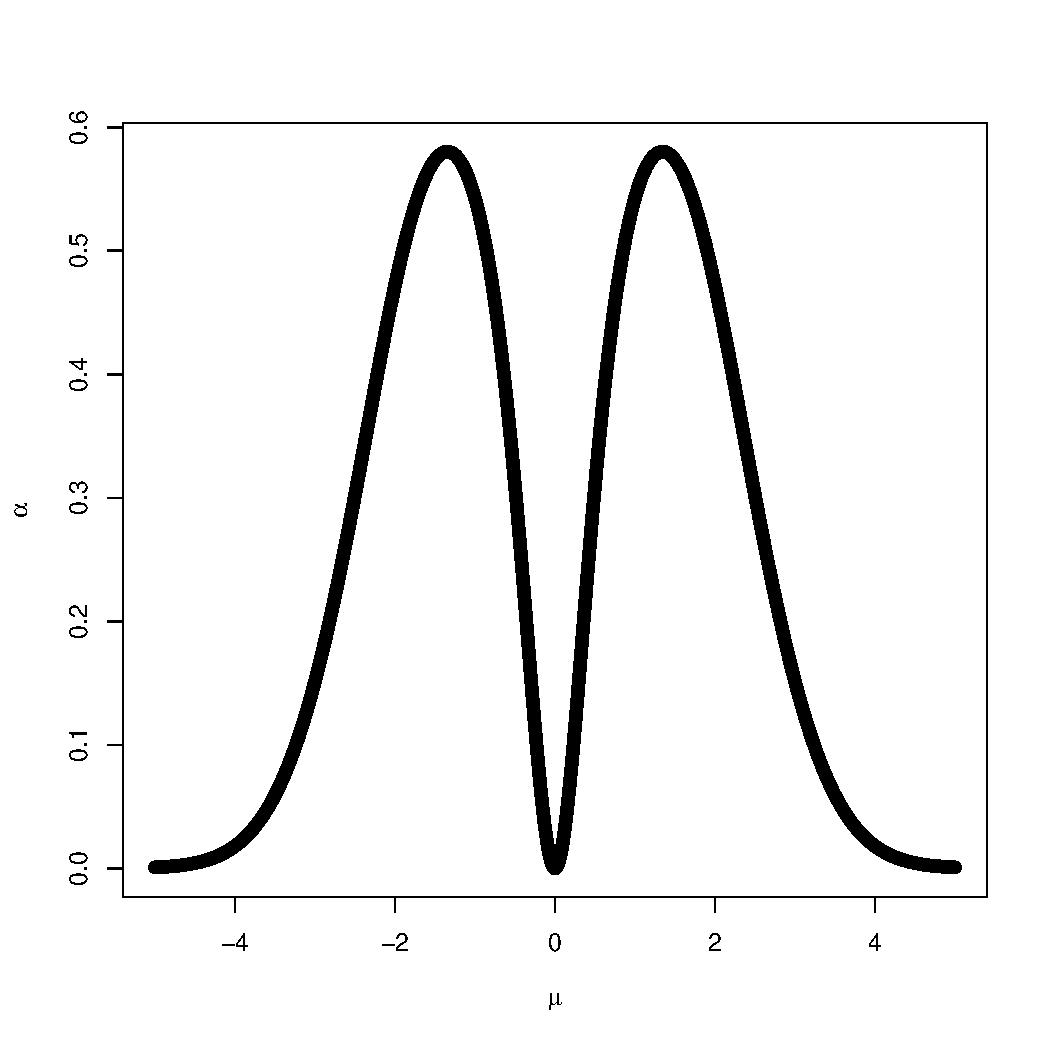
\includegraphics[width=0.5\textwidth]{code/alphaX.pdf}
\label{alphaX}
\caption{The value of $\alpha_X$ necessary to achieve $\alpha=0.05$
  with $\alpha_Y=0.05$ at various values of $\mu$}
\end{figure}

\subsection{Recommendations for Practice}
The estimation and inference for RDDs, under
our framework, takes place entirely for the set of subjects $i\in
\mathcal{W}=\{i: c-b \le R_i \le c+b\}$ for a bandwidth $b>0$.
The first motivation for a choice of $b$ should be substantive: for
which subjects does an effect estimate make sense?
Which subjects could, conceivably, be candidates for treatment?
For instance, in the LSO dataset, it is hardly reasonable to ask what
the effect of academic probation would be on straight-A students.
In the absence of a clear guideline of this sort, a first choice for
$\mathcal{W}$ can be the smallest window that contains substantively
meaningful variation in $R$: this identifies an interpretable group of
subjects.

In addition to $\mathcal{W}$, researchers must pick $f$, a model for $Y_C$.
\citet{gelman2014high} recently argued against using polynomials of
order higher than two.
As a first pass, we endorse that recommendation: higher-order
polynomials are hard to interpret, and it is hard to choose the order
in a non-arbitrary fashion.
For that reason, researchers may start by modeling $Y_C$ as a linear
or quadratic function of $R$.
Visual inspection of a scatterplot of $Y$ against $R$, and possibly
other regression diagnostic tools, can, of course, inform this
choice.

After choosing $\mathcal{W}$ and $f$, researchers will then transform,
and test balance, on a set of covariates that may be informative about
$Y_C$.
As above, a conservative value of $\alpha_X=0.6$ is reasonable,
although other considerations may suggest other values for
$\alpha_X$ (for instance, some confidence in
$f$ and $\mathcal{W}$).
If the balance test rejects, researchers can add more flexibility to
$f$, perhaps by adding polynomial terms, or shrinking
$\mathcal{W}$.
%Additionally, before conducting an outcome analysis, researchers
%should conduct a McCrary Density test \citep{mccrary2008manipulation}.

\citet{rocio} and \citet{angrist2012wanna} both describe a similar data-driven window selection approach:
    use covariates to successively test model specification  for
    windows $\mathcal{W}=\{i: c-b\le R_i\le c+b\}$ for increasing bandwidths $b$.
Then, choose the larges $b$ whose covariate-balance p-value exceeds a pre-specified level.
This approach easily extends to our method, testing balance of transformed covariates at a range of values for $b$.
It is not without its problems, however: p-values at neighboring $b$ values will typically be highly correlated, since they share a large amount of data.
Moreover, multiple-comparison problems can confuse this process, causing idiosyncratically low or high p-values.
The practical consequences of these problems, and whether they may be overcome, is an open statistical question.

\section{Similarities and Differences with Existing RDD Strategies}
\subsection{The Standard Method}
At the highest level, the standard approach to estimating RDDs is identical to what we present here.
Analysts specify and fit a model for $Y_C$ and another model for $\tau$,
The difference between these fitted models, at $R=c$ is the average treatment effect for subjects at $R=c$.
For instance, if the analyst specifies a linear models of $Y_C$ and a constant model for $\tau$, then the procedure reduces to a linear regression:
\begin{equation}\label{standard}
Y_i=\alpha+\beta R_i+\tau Z_i+\epsilon_i.
\end{equation}
\begin{comment}
Researchers skeptical of the linear model can add polynomial $R$ terms, and those skeptical of the constant model for $\tau$ can interact $R$ with $Z$.
\citet{hahn2001iae} show that, under appropriate continuity assumptions, the following estimand is nonparametrically identified:
\begin{equation}\label{late}
\lim_{b\rightarrow 0} \E[Y_T|R\in c\pm b]-\E[Y_C|R\in c\pm b]
\end{equation}
that is, the average treatment effect in the infinitesimal window surrounding $c$.
If researchers can estimate the respective limits of the functions of $r$, $\E[Y_T|R=r]$ and $\E[Y_C|R=r]$, then the difference between their limits, as $r\rightarrow c$ is equal to the estimand (\ref{late}).
To this effect, \citet{porter2003estimation} suggested using local linear regression to estimate the limits, and \citet{imbens2012optimal} and \citet{desjardins2008impact} have provided optimal bandwidths for the local linear regression.
In fact, \citet{imbens2008regression} pointed out that regressing $Y$ on $R$, $Z$, and $R:Z$, using only data in a window around the cutoff, is similar in spirit, nearly as good, and substantially easier than the estimator in \citet{porter2003estimation}.
\end{comment}

The standard approach to RDDs differs in two important ways from the method we describe here.
First, the source of identification: in the standard approach, identification comes from the continuity of the expected values of $Y_T$ and $Y_C$, as $R$ varies---this allows researchers to estimate their values at the cutoff and estimate the treatment effect there.
In contrast, our method relies more heavily on the local randomization assumption: that, after transforming $Y_C$ values, treatment assignment may be modeled as random.
For this reason, a discrete $R$ may pose a problem for the
conventional approach; our method avoids this issue.
See, however, \citet{lee2008regression} which explicitly addresses
discrete $R$.

The estimand standard approach is a limit of average treatment effects in ever-tightening windows.
This can be difficult to interpret.
In some scenarios, it may be possible to interpret as the average treatment effect for subjects for whom $R=c$; however, this will often differ from the researcher's estimand of interest.
Our estimand is simply the function $\tau=\g(R;X)$---the function describing the treatment effect for subjects in the window $\mathcal{W}$.

Perhaps surprisingly, the standard estimator coincides with our estimator in one particular setting.
If analysts use (\ref{standard}) to estimate $\tau$, and, in a different analysis, model $Y_C$ as linear, model $\tau$ as constant, and use the difference in means between treatment and control subjects as a test statistic, the two estimates will be identical.
We formalize this in the following proposition:
\begin{prop}
If, in $\mathcal{W}$, a researcher uses OLS to model $Y_C=f(R)+\epsilon=\beta R +\epsilon$ and $\tau=\tau_0$, and takes as the test statistic $\bm{\ych'Z}$, then the Hodges-Lehmann estimate of $\tau_0$ will be equal to the OLS estimate of $\tau$ from the regression (\ref{standard}), fit using the data in $\mathcal{W}$.
\end{prop}
The proof to this proposition is basically the same as an argument from \citet[][ p. 290]{rosenbaum2002covariance}
\begin{proof}
Let $\mathcal{R}$ be the matrix formed by joining a column of ones to
$\bm{R}$. Then let
$H=\mathcal{R}(\mathcal{R}^T\mathcal{R})^{-1}\mathcal{R}')$. Under $H_{\tau_0}:Y_{Ti}-Y_{Ci}=\tau_0$,
$\ych_{\tau}=(I-\mathcal{H})(Y-Z\tau)$ and the test statistic is
$Z^T\ych_\tau=Z^T(I-\mathcal{H})(Y-Z\tau)$. When $\tau=\tau_0$, the expected value of the
test statistic is $\E Z^T \ych=\E Z\E \ych=0$ since
$\mathcal{R}$ contains a constant term and the model is fit with OLS.
The Hodges-Lehmann estimate of $\tau$, solves the equation
\begin{align}
Z^T\ych_\tau&=0\\
Z^T(I-\mathcal{H})(Y-Z\tau)=0
\end{align}
which is solved when
$\tau=\frac{Z^T(I-\mathcal{H})Y}{Z^T(I-\mathcal{H})Z}$, which is equal
to the OLS estimate of the coefficient of $Z$ from the regression of
$Y$ on a constant, $R$, and $Z$.
\end{proof}
That is, one of the simplest conventional RDD estimates can be
re-interpreted as a Hodges-Lehmann estimate of a constant treatment
effect under transformed ignorability.
In this case, rather than provide a new method, we reinterpret the
conventional method.

\subsection{Local-Randomization-Based Inference (\citealt{rocio})}
\citet{rocio} developed a randomization-based approach to RDDs. Their
approach was to limit the data to a small window around the cutoff,
analogous to our $\mathcal{W}$, and argue that within $\mathcal{W}$,
subjects are for practical purpose, randomized into treatment and
control groups, so $Z \independent Y$.
As we mentioned above, this corresponds to the case where one ``models''
the relationship between $Y_C$ and $R$ with a constant function---that
is, assumes no relationship between $Y_C$ and $R$---in $\mathcal{W}$,
in which case transformed ignorability is equivalent to standard
ignorability (\ref{superIgnore}).

We argued above that in many instances the relationship between $R$
and $Y_C$ is both strong and important, so ignoring it, even in a
small window $\mathcal{W}$, can yield misleading results.
That being said, the randomization-based approach in \citet{rocio} has
some advantages over the more general approach here.
To wit, \citet{rocio}'s set-up allows researchers to estimate a broader class of estimands.
For instance, if one models the data in $\mathcal{W}$ as arising from
a randomized experiment, one may estimate quantile treatment effects
or displacement effects \citep{rosenbaum:2001}.
Estimating these in the framework we have developed here requires a
non-trivial extension.

\subsection{Conditional Ignorability Assumption (\citealt{angrist2012wanna})}
\citet{angrist2012wanna} addressed the question of estimating
treatment effects away from the cutoff with a new assumption, called
the ``Conditional Ignorability Assumption,'' or CIA.
The assumption states that, conditional on covariates $X$, treatment
assignment is mean-independent of the running variable.
This approach shares three important similarities with ours.
First, it explicitly formulates causal identification in terms of an
ignorability assumption.
Second, it is interested in effects for a sample of subjects which is
not asymptotically vanishing.
Finally, it uses covariates to justify causal identification away from
the cutoff.

In its details, though, it is quite different---its identification
assumption is different from ours, as is the method it proposes.
Unlike our approach,
CIA assumes mean independence, which is sufficient for unbiased estimation but not
inference.
Therefore, for estimation, CIA may be weaker than Transformed
Ignorability, but for inference it requires some stronger assumptions.
Additionally, covariates are explicit in the definition of CIA, but
not in Transformed Ignorablility.
Both assumptions seek to make $R$ ignorable---Transformed Ignorability
does so with modeling, while CIA does so with covariates.


\section{Example: The Effect of Academic Probation}


\begin{figure}[htb]
\centering
\mbox{
\subfigure[]{\includegraphics[width=.45\textwidth]{graphics/figure2_1.pdf}}
\quad
\subfigure[]{\includegraphics[width=.45\textwidth]{graphics/hs_gpa.pdf}}
}
\caption{(a) The RDD from LSO. The first-year GPAs were shifted so
  that the cutoff is at zero---that is, each campus's
 cutoff was subtracted from its students first-year GPAs. Subsequent
 GPA was averaged according to first-year GPA. (b) Students
 log-transformed high-school GPAs, also averaged by first-year college
 GPAs.}
\label{LSO}
\end{figure}

\citet{lindo2010ability}---LSO---attempted to estimate the effect of
academic probation (AP) on college students at an unnamed
Canadian university.
One of the outcomes that LSO measures is $nextGPA$, students'
subsequent GPAs, either for the summer or fall term after students'
first years.
Figure \ref{LSO} (a) displays $nextGPA$ as a function of students'
first-year GPAs.
Their causal question of interest is whether AP causes a change in
$nextGPA$: do students on AP tend to have higher (or lower) subsequent
GPAs?
Recall that AP is determined almost exclusively\footnote{There are 48
  cases, out of a total of 44,362, where students were not put on AP
  despite GPAs below the cutoff, and three cases in which students
  were put on AP despite having GPAs above the cutoff. In this paper,
  as in LSO, we will follow the ``intent to treat'' principle and
  estimate the effect of treatment \emph{assignment}---that is, having
  a GPA below the cutoff---instead of actual treatment (AP). Since the
  number of cases in which these two disagree is such a small
  proportion of the total, we anticipate that this will have a minimal
  impact on our estimates.}
by first-year cumulative GPA, which in this case is the running
variable $R$.
That is, students with GPAs below the cutoff are ``treated'' with AP,
and students above the cutoff are in the control group.
The university in question has three campuses, two of which have
cutoffs of 1.5; the other has a cutoff of 1.6.
To combine data from the three schools, LSO centered each student's
first-year GPA at the appropriate $c$, so $R_i$ is a student $i$'s
first year GPA, minus the cutoff at his college.
Then, $Z=\indicator{R\le 0}$

A relevant region in which to estimate a treatment effect is within
$0.3$ grade-points of the cutoff $c$.
Conventionally, $0.3$ represents the difference in grade points
between a C, say, and a C-, or any other grade half-step.
As a first pass at $\mathcal{W}$, then, we will look at
$\mathcal{W}_1=\{i:R_i\in [-0.3,0.3]$.
A first pass at $f$ will be $f_1(R_i)=\alpha +\beta R_i+\epsilon_i$, a
linear function.
Simplicity recommends a linear approximation, and an examination of a
scatterplot of $Y$ versus $R$ suggests that it will be a close
approximation in $\mathcal{W}$.



To test $f_1$ and $\mathcal{W}_1$, we will conduct placebo tests,
examining balance of transformed covariates.
LSO exploits seven pre-treatment variables to test the RDD assumptions
in the AP case: high-school GPA (available, for some reason, on a
scale from 0--100), the total number of credits attempted in
students' first year and students' age at college entry, which are
continuous, and dummy variables for campus (the university has three
campuses), whether students'
first language is English, and whether
students were born in North America.
Figure \ref{LSO} (b) displays the logit of students'
high-school GPAs, which had been on a 1--100 scale
suggests that the curvature in relationship of (transformed)
high-school GPA with $R$ is greater than $nextGPA$, suggesting that
high-school GPA may be a good candidate for a conservative placebo
test.
\citet{hansen:bowers:2008} suggested an omnibus statistic
for testing covariate balance; their routine, implemented as
\verb|xBalance| in the \verb|R| package \verb|RItools| \citep{bowers2010ritools,rcite}, yields a p-value of
$p=$0.03, well above the 0.6 threshhold.


\begin{comment}
Another important specification test for RDDs is the McCrary density test \citep{mccrary2008manipulation}.
It is designed to test whether subjects consciously sort around the cutoff by manipulating their $R$ values explicitly.
It does so by examining whether an unexpectedly large or small number of subjects find themselves just barely on one side of the cutoff or the other.
A McCrary test failure is neither necessary nor sufficient to show that subjects sorted around the cutoff; however, it is deeply suspicious.
In the LSO data, in $\mathcal{W}$, the McCrary p-value was 6.8e-08, so some amount of sorting seems likely.

AP is certainly a dubious distinction, and many students will try to avoid it.
\end{comment}


With $f_1$ and $\mathcal{W}_1$ in hand, we can test Fisher's %'
$H_0: Y_{Ci}=Y_{Ti}$ for all subjects $i$.
Using the same testing procedure as the covariate placebo test, \verb|xBalance|,
the p-value is 0.0092, which rejects $H_0$ at level $\alpha=0.05$.

To estimate the magnitude of the effect, we need, additionally, a model $\g$ for treatment effects.
Examination of Figure \ref{LSO} suggests that the slope relating $R$
to $nextGPA$ does not shift from one side of $c$ to the other, so a
constant effect model may be sufficient.
Inverting the hypothesis test for a range of constant effects
yields a 95\% confidence interval of 0.05--0.38,
with a Hodges-Lehmann point estimate of 0.21.

\begin{figure}
  \centering
  \includegraphics[width=0.8\textwidth]{graphics/dim2.jpg}
  \caption{Confidence regions for $\nu$ and $\tau$ from model (\ref{complexTau}). The green region is a 90\% confidence region, the yellow is 95\% and the red is 99\%.}
  \label{dim2}
\end{figure}

It may be, though, that the effect of AP varies with first-year GPAs.
Students with higher GPAs may be more motivated than their lower-GPA
colleagues, and therefore respond more heartily to the threats that
accompany AP.
This suggests a more nuanced model for $\tau$:
\begin{equation}\label{complexTau}
  \tau_i=\g(R_i; \bm{\phi})=\tau_0+\nu R_i
\end{equation}
Where the treatment effect $\tau$ is decomposed into $\tau_0$, a
constant effect for all students, and
$\nu$, an effect that varies linearly with $R$.
That is, $\bm{\phi}=\{\tau_0,\nu\}$.
Test statistics that focus only on the relationship
between hypothetical values for $Y_C$ and $Z$ will perform poorly when
testing a hypothesis that involves both $Z$ and $R$, as in
(\ref{complexTau}).
This is especially true for test statistics that are sensitive to
location shifts, such as the Wilcoxon test or the
\verb|xBalance| procedure that we have used so far: for
each hypothetical $\tau_0$, a hypothetical $\nu$ is available so that
transformed, hypothetical values for $Y_C$, that is,
$\ych_{\tau_0,\nu}$, have the same locations in both treatment and control groups.
An appropriate test statistic for (\ref{complexTau}) is sensitive to
differences in both the slope and the intercept of the $\ych_{\tau_0,\nu}$-$R$
regression lines between the treatment and control groups.
One such statistic is the omnibus F-statistic from the regression of
$\ych_{\tau_0,\nu}$ on $R$, $Z$, and $R:Z$.
Inverting the permutation test of this statistic yields the confidence
region in Figure \ref{dim2}.
Marginally, the inference for $\tau_0$ is roughly the same as the constant effects
model above, but the data are, somewhat surprisingly, uninformative
about $\nu$.

\subsection{Robustness Checks}

The choices we made for $b$ and for $f$ could have been made
differently; they were motivated, respectively, by substantive
background and a desire for simplicity, and were validated with
covariate placebo tests.
That being the case, it may be wise to examine the robustness of our
analysis to different choices for $b$ and $f$.

A reasonable alternative for $f$ allows $Y_C$ to vary with $R$ as a
quadratic polynomial, so $Y_{Ci}=f(R_i)=\beta_0+\beta_1 R_i+\beta_2
R_i^2$.
Using this quadratic model for $f$ leaves our inference, in this case,
virtually unchanged: a p-value of 0 for $H_0$, a confidence
interval of 0.04--0.39, and a Hodges-Lehmann
point estimate of 0.22.

% latex table generated in R 3.1.0 by xtable 1.7-3 package
% Thu Sep 18 12:07:37 2014
\begin{table}[ht]
\centering
\begin{tabular}{rllll}
  \hline
 & b & p-value & 0.95 CI & HL Estimate \\ 
  \hline
main & 0.3 & 0.0092 & (0.05,0.38) & 0.21 \\ 
  DataDriven & 1.03 & 1.2e-10 & (0.17,0.33) & 0.25 \\ 
  IK & 1.25 & 5.8e-16 & (0.2,0.33) & 0.26 \\ 
   \hline
\end{tabular}
\caption{Null Hypothesis p-values, 95\% confidence intervals, and Hodges-Lehmann point estimates for a variety of bandwidths in the LSO data.} 
\label{bandwidths}
\end{table}
To examine robustness to choices of bandwidth $b$ and hence
$\mathcal{W}$, we tried two alternative bandwidths.
The results are summarized in Table \ref{bandwidths}.
First, a data-driven bandwidth, using a procedure similar to what was
suggested in \citet{rocio}: setting $b$ to the largest value for which
a covariate placebo test yields a p-value above $\alpha_X=0.6$.
The largest $b$ for which this is true turns out to be $b=1.03$; at this bandwidth, the p-value for a covariate placebo test is 0.
This yields a p-value for $H_0$ of 1.2e-10, a confidence interval of 0.17--0.33 and a point estimate of 0.25.
Finally, \citet{imbens2012optimal} suggests a procedure for choosing a bandwidth that minimizes mean-squared-error for the conventional local-linear RDD analysis.
We implemented this method, specifying a ``rectangular" kernel (weighting equally all observations within the window, and assigning all others a weight of zero) using the \verb|rdd| package in \verb|R| \citep{Rcite,rdd}. %"
In the LSO case, that procedure yields a bandwidth of 1.25, with a covariate balance p-value of 0.
The \citet{imbens2012optimal} bandwidth yields an $H_0$ p-value of 5.8e-16, a 95\% confidence interval of 0.2--0.33, and a point estimate of 0.26.
These results suggest an insensitivity to the choice of $b$.

\subsection{LSO Results from Other Methods}
% latex table generated in R 3.1.0 by xtable 1.7-3 package
% Thu Sep 18 12:07:44 2014
\begin{table}[ht]
\centering
\begin{tabular}{rllll}
  \hline
 & b & p-value & 0.95 CI & HL Estimate \\ 
  \hline
main & 0.3 & 0.0092 & (0.05,0.38) & 0.21 \\ 
  Conventional & 0.79 & 7.5e-15 & (0.17,0.29) & 0.23 \\ 
  CFT & 0.16 & 3.2e-05 & (0.07,0.18) & 0.12 \\ 
   \hline
\end{tabular}
\caption{Null Hypothesis p-values, 95\% confidence intervals, and point estimates for our main analysis, compared with the analysis in Cattaneo, et al. (2014), and the conventional local-linear estimate with the Imbens and Kalyanaraman (2012) bandwidth.} 
\label{alt}
\end{table}
How does our method compare with others in the LSO analysis?
To see, we use the \verb|rdd| package in \verb|R| \citep{rdd} to
implement the latest limit-based RDD analysis.
This used a local linear regression, with the bandwidth recommended by \citet{imbens2012optimal} (this time with the recommended ``triangular'' kernel), to estimate the effect of AP at the cutoff.
Next, we implemented the randomization-based routine recommended in \citet{rocio}.
First, to choose a bandwidth, we used the \verb|xBalance| function to examine covariate balance---without transformation---at a range of bandwidths near the cutoff.\footnote{\citet{rocio} recommends testing balance separately for each covariate, and choosing the minimum p-value at each possible bandwidth. We found this to be overly conservative---it rejected the null hypothesis at every possible bandwidth, due, possibly, to multiple comparisons.}
The highest bandwidth that corresponded to a p-value greater than $\alpha_X=0.15$, which they recommend, was $b=0.15$.
Then, we used \verb|xBalance| as a difference-in-means test to test the strict null hypothesis within the window, and we inverted it for a 95\% confidence interval and a Hodges-Lehmann point estimate.

Our method gives roughly the same estimate as the conventional, local linear approach, though with a wider confidence interval.
The \citet{rocio} method gives a slightly different answer; in fact, the estimates from our method and from the conventional method are outside the randomization-based method's confidence interval.%'
This may be because \citet{rocio} ignores the relationship between $nextGPA$ and $R$.
The general trend---higher $nextGPA$ for higher $R$---is in the opposite direction as the effect of AP---students with lower $R$ are treated, and experience a positive effect.
These two factors may partially cancel each other out, leading to a point estimate that is biased toward zero.
If this is the case, it illustrates the importance of explicitly modelling $R$ in an RDD analysis.

\subsection{Other Issues in the LSO Dataset}
Our analysis of the LSO dataset is intended as an illustration of our novel RDD analysis method; as a study of the effect of AP, it is incomplete.
In particular, there are two serious statistical issues that we ignored, for the sake of brevity.
We mention them briefly here.
First, 4.39\% of the subjects in the LSO dataset were missing a GPA either for their first-semester, their subsequent semester, or both.
Our analysis implicitly treated these subjects as missing completely at random; however, this assumption may not be true.

More importantly, perhaps, are the results of a McCrary density test
\citep{mccrary2008manipulation}, which yielded a p-value of
6.8e-08, indicating that some subjects may have manipulated their
first-year GPAs to avoid AP.
In an analysis not shown here, but available upon request, we found
suggestive evidence that a number of students may have dropped a
course in order to achieve a GPA just above the cutoff.
In fact, if we remove the students at the cutoff who took only four
(the mode is five), the McCrary p-value increases to 0.34.
Removing these students has negligible effect on our estimates or inferences.
The justification for this maneuver is debatable, and doing so here
would distract from our central point; suffice to say that, from a
substantive perspective, the LSO result needs further investigation.

\section{Conclusion}
This paper presents a novel interpretation and modeling approach to
regression discontinuity designs.
The new approach has some advantages over the conventional approach,
including natural interpretation and statistical inference when the
running variable is discrete or the the sample size is small,
identifying assumptions that speak to the link between RDDs and
randomized experiments, and a role for covariates in validating inference.

The approach presented here may have some weaknesses as well.
Firstly, it requires a set of covariates in the data whose relationships to the outcome of interest are similar to the running variable $R$'s.
Not only are such covariates not always available, but even in a rich dataset it may be hard to assess the covariates' usefulness.
Secondly, there may be some scenarios in which the conventional RDD assumptions are more plausible than those presented here.
Finally, in the study of academic probation that we discuss here, our method
yielded a wider confidence than the conventional method.
It is unclear if this will generally be the case.

Though starting from a similar point, this paper's approach differs in
some important ways from the approach in \citet{rocio}.
That paper suggests assuming that subjects in a window close to the
cutoff are randomized, with equal probabilities, to various treatment
conditions.
In particular, within the window of analysis, the potential outcomes
are not related to treatment assignment---and, therefore, the running
variable $R$.
In contrast, this paper allows a relationship between potential
outcomes and $R$ in the window of analysis.
The question of which set of assumptions is more plausible will depend
on the substantive question of interest.
\citet{rocio}'s approach allows more flexibility in the choice of
estimands, whereas the approach here is limited to estimating
mean-based estimands.
This paper's approach will hopefully be attractive to researchers who
are drawn to randomization-based arguments, but are reluctant to
abandon the familiar trappings of the conventional RDD approach.

Recently, the RDD methodology literature has begun to address the case
of multiple running variables \citep{papay2011extending,
  reardon2012regression}.
The method we present here extends to that case in a straightforward
way, using multivariate modeling techniques to disentangle outcomes
from the running variables and joint permutation tests for inference.

Finally, this paper highlights the need for future work on choosing a
window of analysis based on a sequence of specification tests.

\bibliographystyle{plainnat}
\bibliography{/Users/acsales/causalinference}
\end{document}

First, $Y_{Ci}=f(R_i;\bm{\theta})+\epsilon_i$, is a model relating $Y_C$ to $R$, where $\bm{\theta}$ is a set of parameters to estimate.
Here, $\epsilon_i$ may be modeled as either drawn from a random population or fixed; in the latter case, the model fit $f$ can be thought of as algorithmic, as opposed to probabilistic, in the sense of \citet{rosenbaum2002covariance}.
For example, one may model $Y_{Ci}=\alpha+\beta R_i +\epsilon_i$, a linear model.
A simpler example is $Y_{Ci}=\epsilon_i$, in which there is no
relationship between $R$ and $Y_C$; in this case, our method reduces
to the method described in \citet{rocio}.

One approach to effect estimation in this framework begins by
specifying a model for the treatment effect.

In practice, researchers do not have access to the entire vector
$Y_C$, so instead they must propose hypotheses $H_{\bm{\phi}}$,
yielding $\tilde{Y}_C$, and evaluate those assumptions relative to
transformed ignorability.
